\chapter{Significance of \jwone and \jwtwo for GK stars}\label{chap:RESULTS}
% ==========================================
\section{Possible origins of dwarf-giant color separation}


We identify by eye that \jwone and \jwtwo present a significant separation in color between dwarfs and (sub-)giants for all G and early K spectral types. This trend in \jwone and \jwtwo with luminosity class for G and early K dwarfs may extend to later spectral types (M stars), but the limited number of M dwarfs in the Michigan Spectral Atlases precludes a robust determination \ref{sec:CONCLUSION}.

The separation is approximately one robust standard deviation of the colors for a given spectral type and luminosity class. For example, the color distribution of G5V stars is $J-W2=0.405\pm0.078$, for G5III stars is $J-W2=0.573\pm0.055$, a difference of $0.168\pm0.095$ of more than one standard deviation. While there is significant overlap in the colors of stars of different luminosity classes, this still permits a probabilistic assignment of luminosity class which we explore further in ${\S}5$.

The robust standard deviation of the colors of a given spectral type and luminosity class in the spectral type range of interest (G0-K5) is consistent with typical WISE and 2MASS magnitude measurement uncertainties ($\sim$0.05--0.15 mag). Thus, this implies the overlap in the dwarf-giant color distributions may be due to measurement uncertainties rather than a physical origin.  More precise color measurements may increase the statistical significance of this separation between dwarfs and (sub-)giants in color.

In the next sections, we turn to highlighting sample applications of this utilizing this primary result for use in distinguishing dwarfs from giants.
\begin{figure}
    \centering
    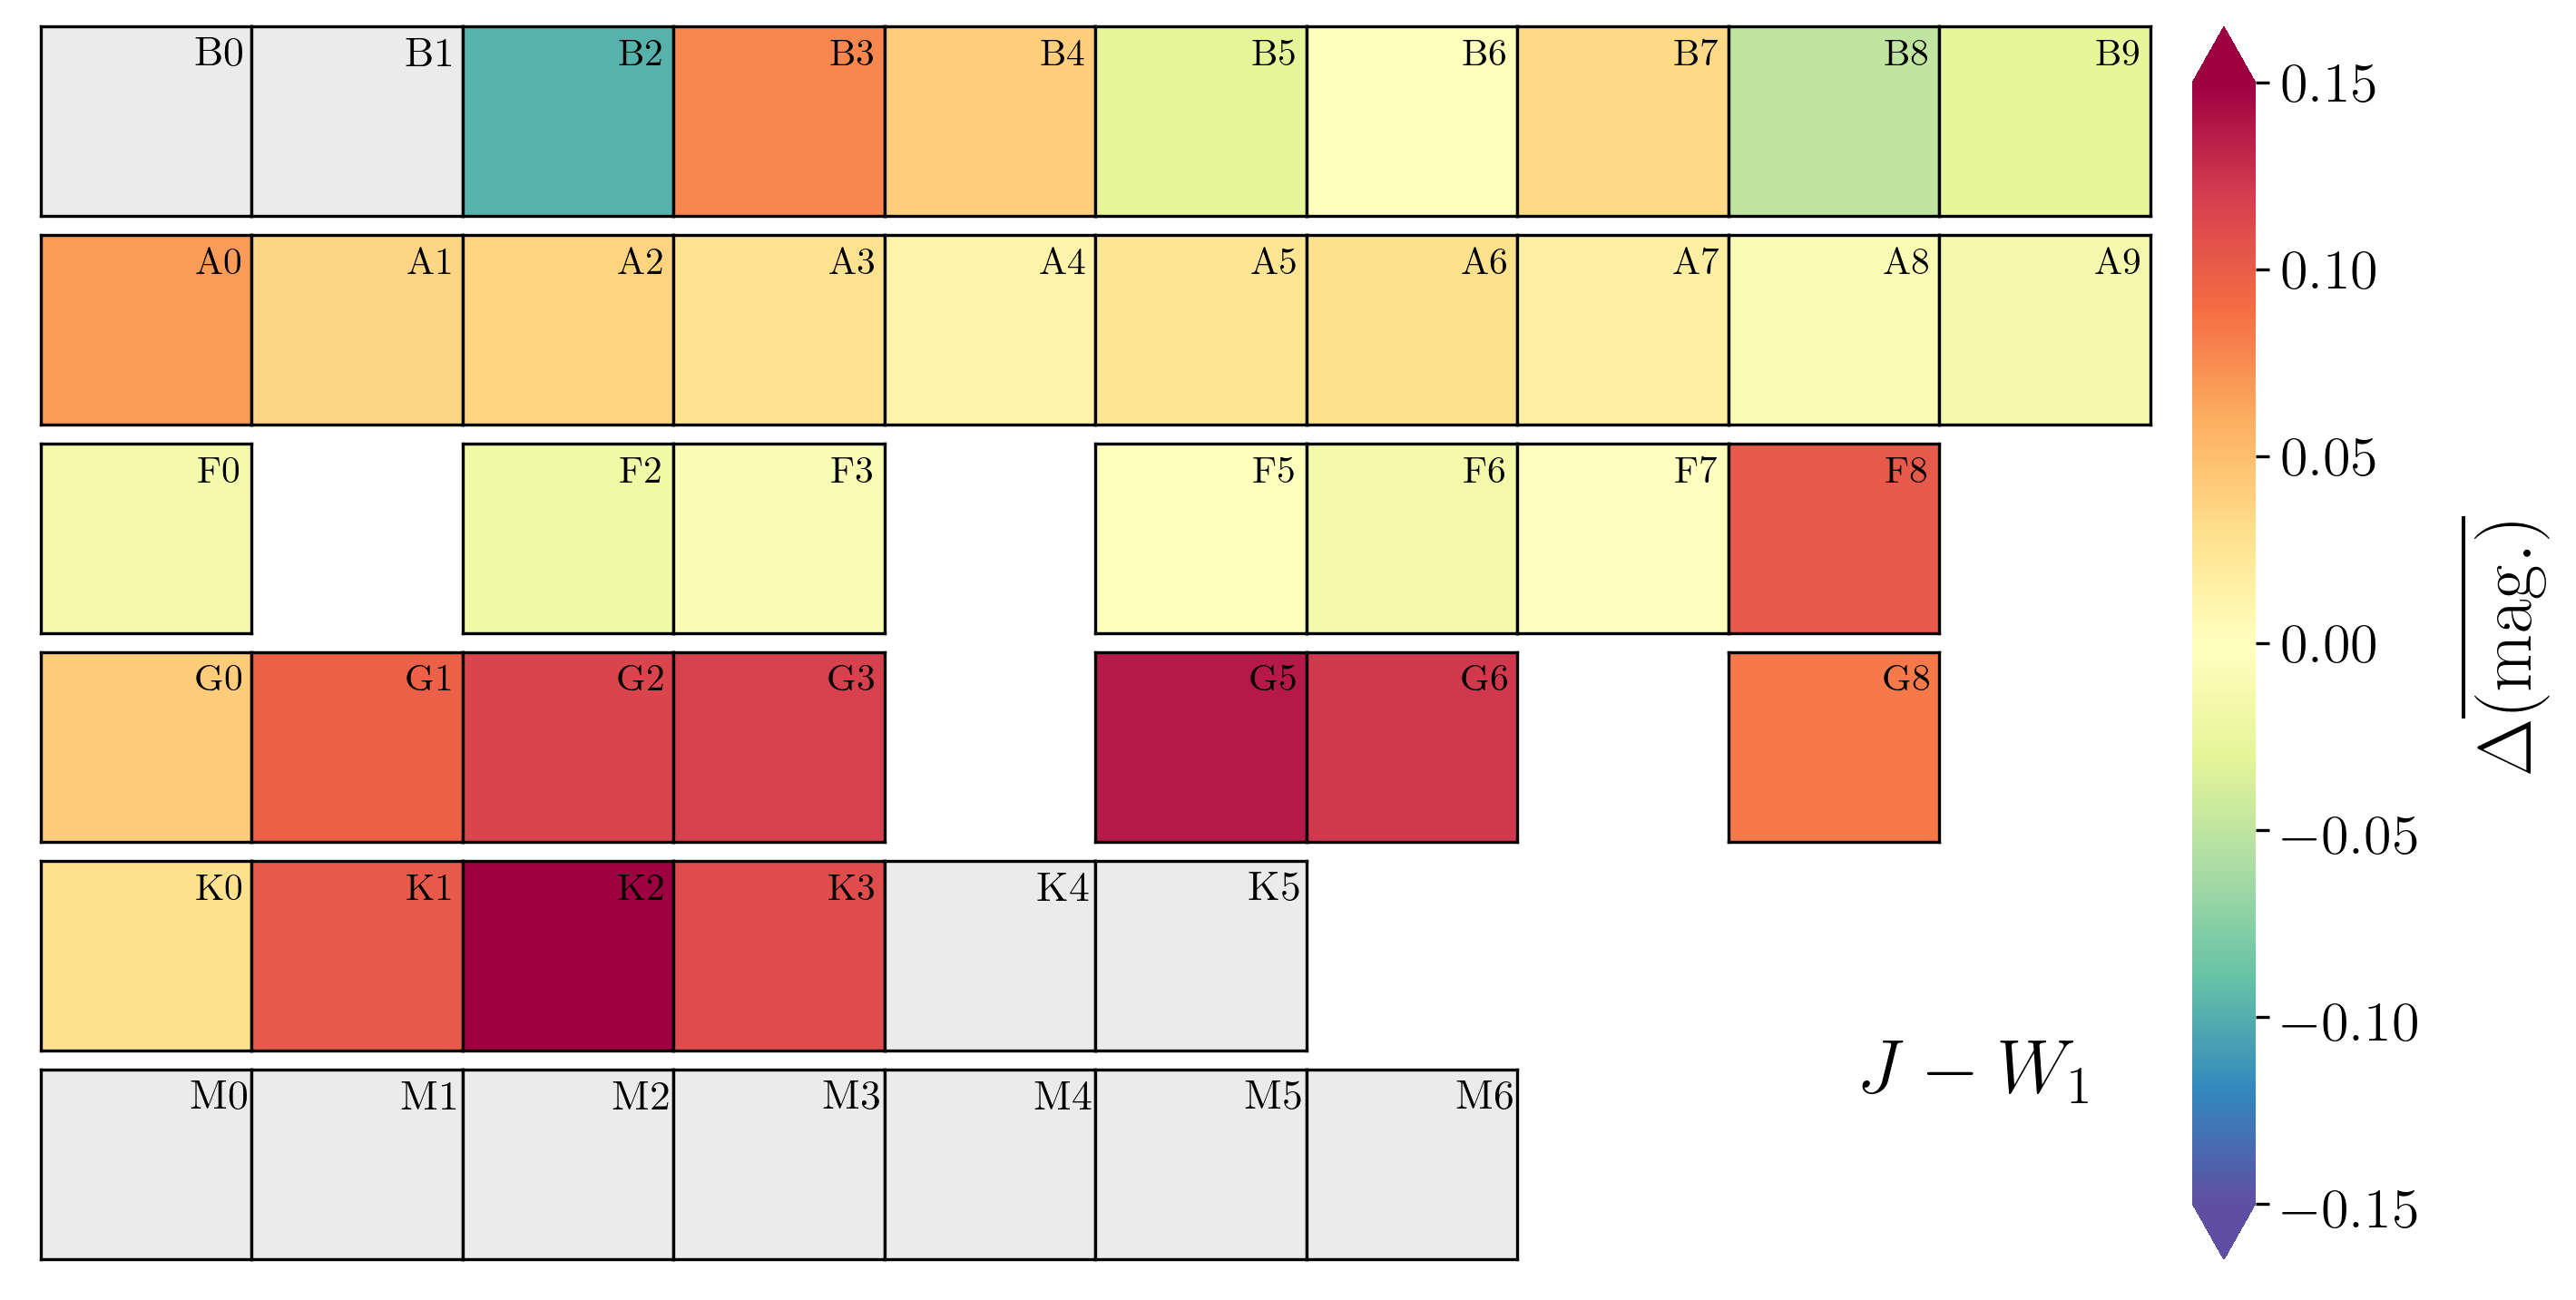
\includegraphics[width=1.0\textwidth,clip=true]{Figures/periodic/periodic-delta_J_W1.png}
    \caption{Caption}
    \label{fig:periodic-delta-jw1}
\end{figure}

\begin{figure}
    \centering
    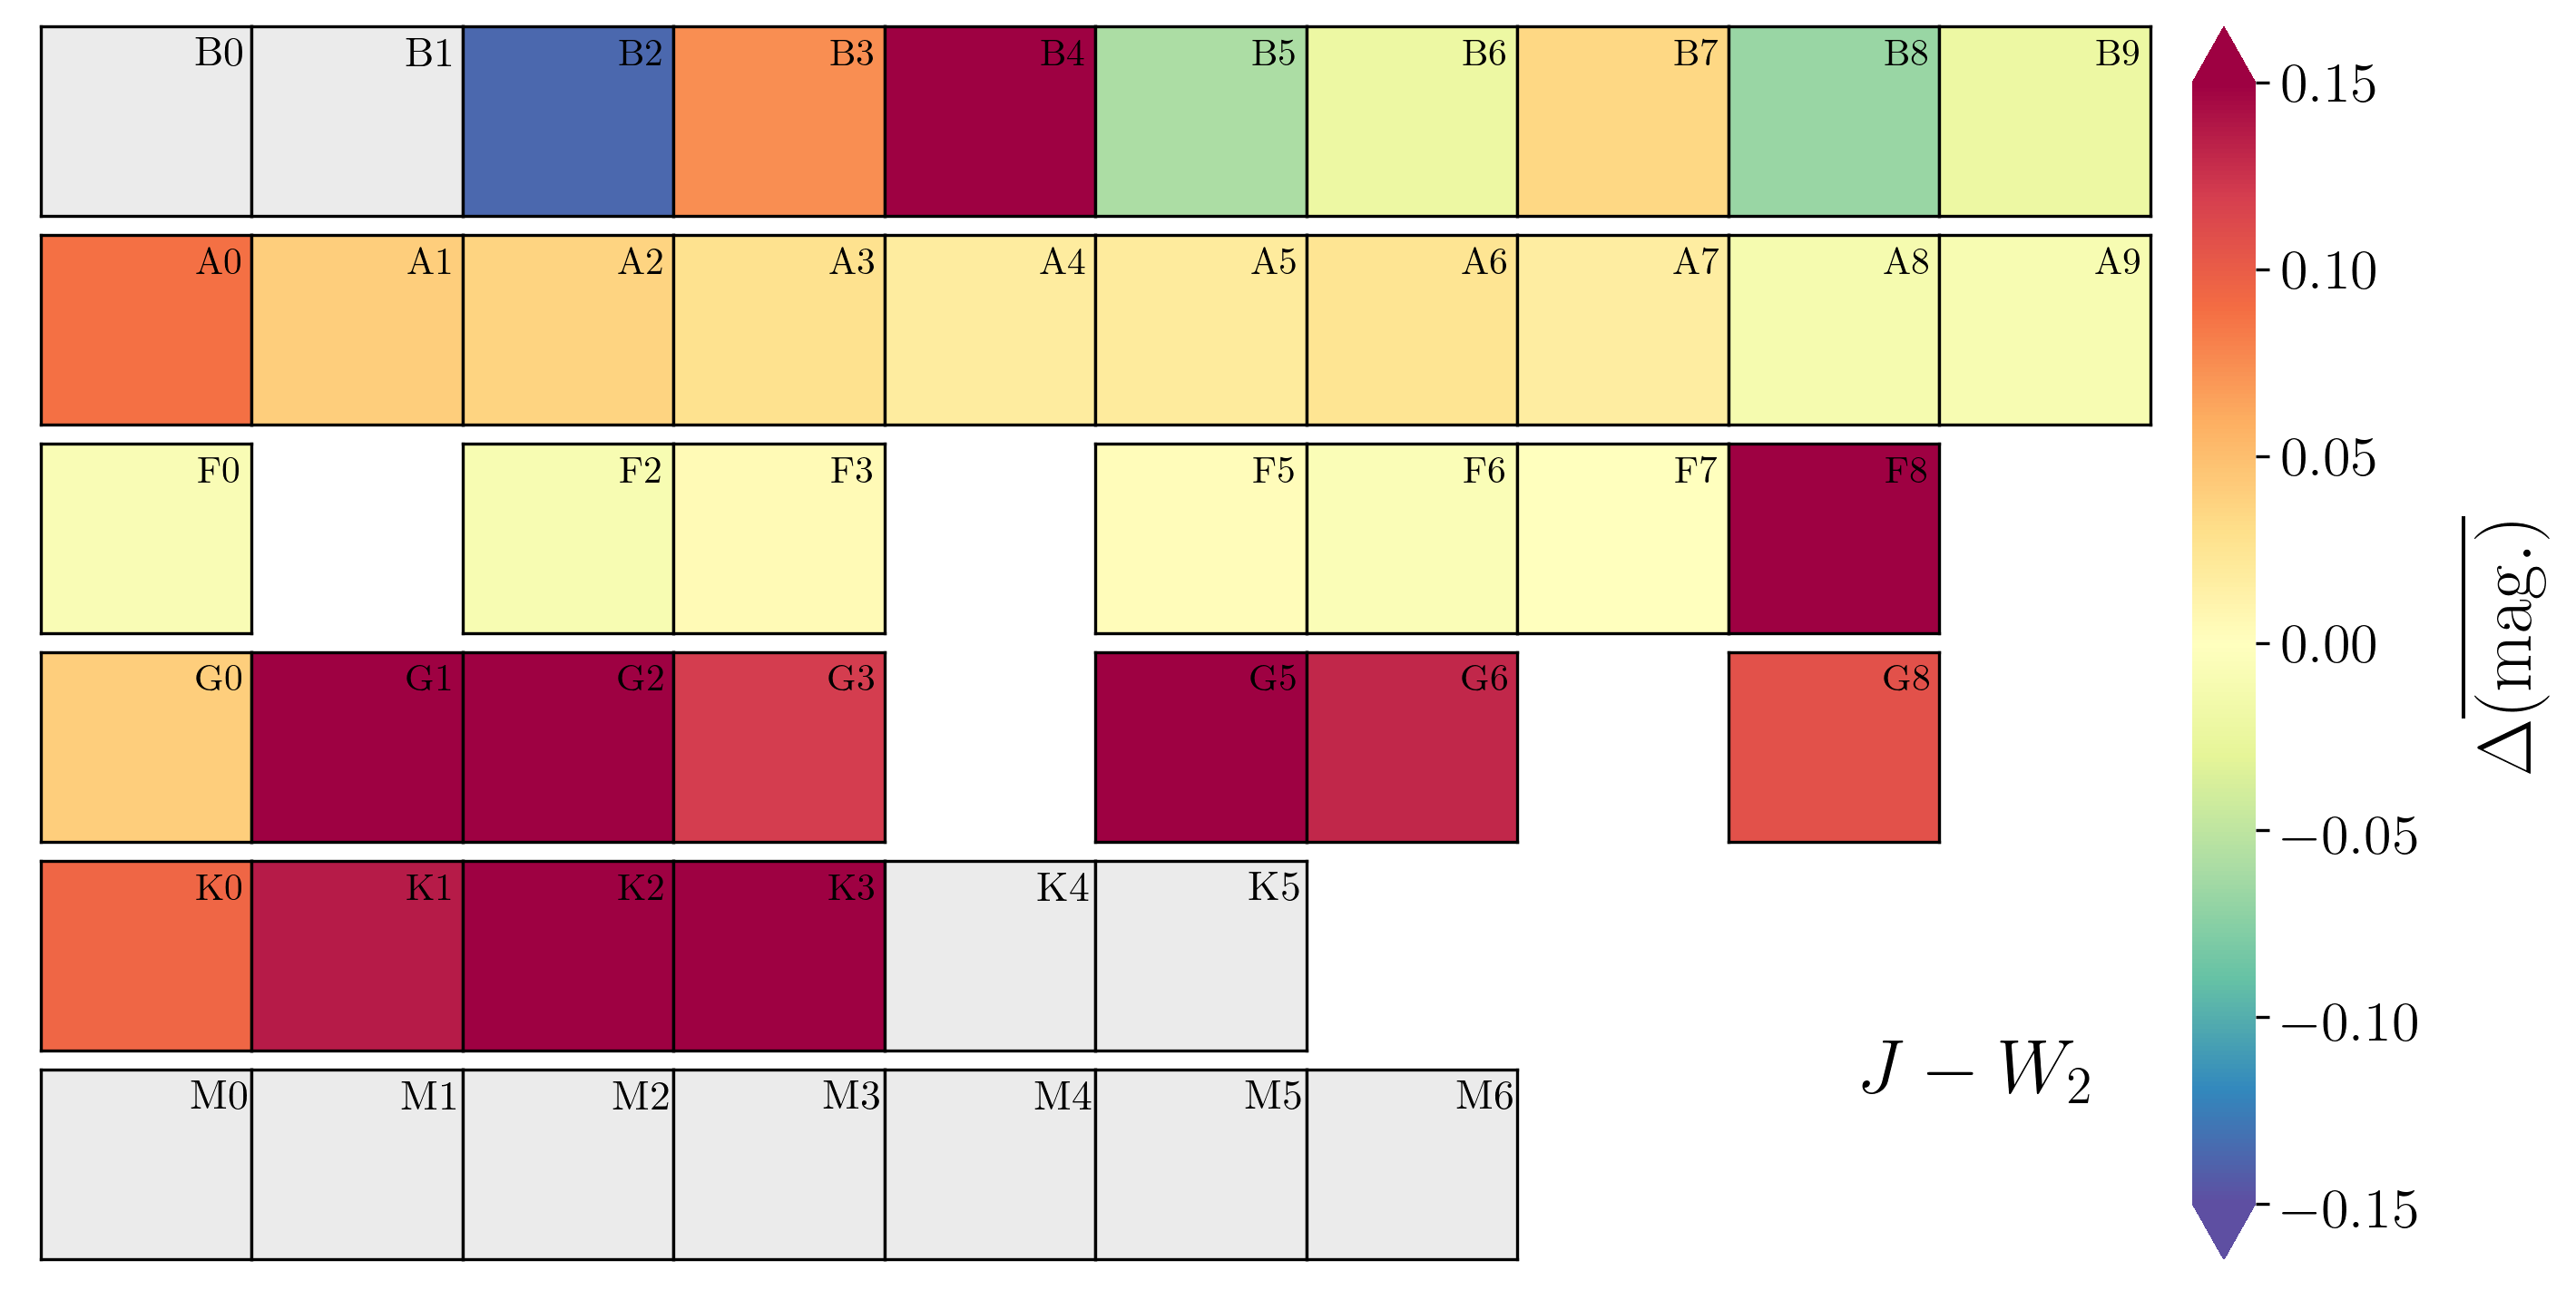
\includegraphics[width=1.0\textwidth,clip=true]{Figures/periodic/periodic-delta_J_W2.png}
    \caption{Same as Figure \ref{fig:periodic-delta-jw1}, but for \jwtwo.}
    \label{fig:periodic-delta-jw2}
\end{figure}

\section{Sample applications}
\subsection{Reduced proper motions}
\subsection{Galactic population model}

All of the Michigan stars are HD stars with GAIA parallaxes and proper motions.  We cross-correlate the Michigan catalog with the GAIA First Data Release \citep[]{gaia1,gaia2,Lindegren2016}.  In Figure 8, we plot the standard reduced proper motion (${rpm}_J$) for the Michigan stars as a function of \jwtwo for spectral types from G0--K5 and luminosity class, using GAIA proper motions.  In Figure 9, we plot the Absolute J-band magnitudes for the Michigan stars as function of \jwtwo for spectral types from G0--K5 and luminosity class, using GAIA parallaxes.

From these plots, we see that the classification success rate of the Michigan catalog is high, but not perfect (e.g. luminosity class IV 


\begin{figure*}[t]
  \begin{center}
      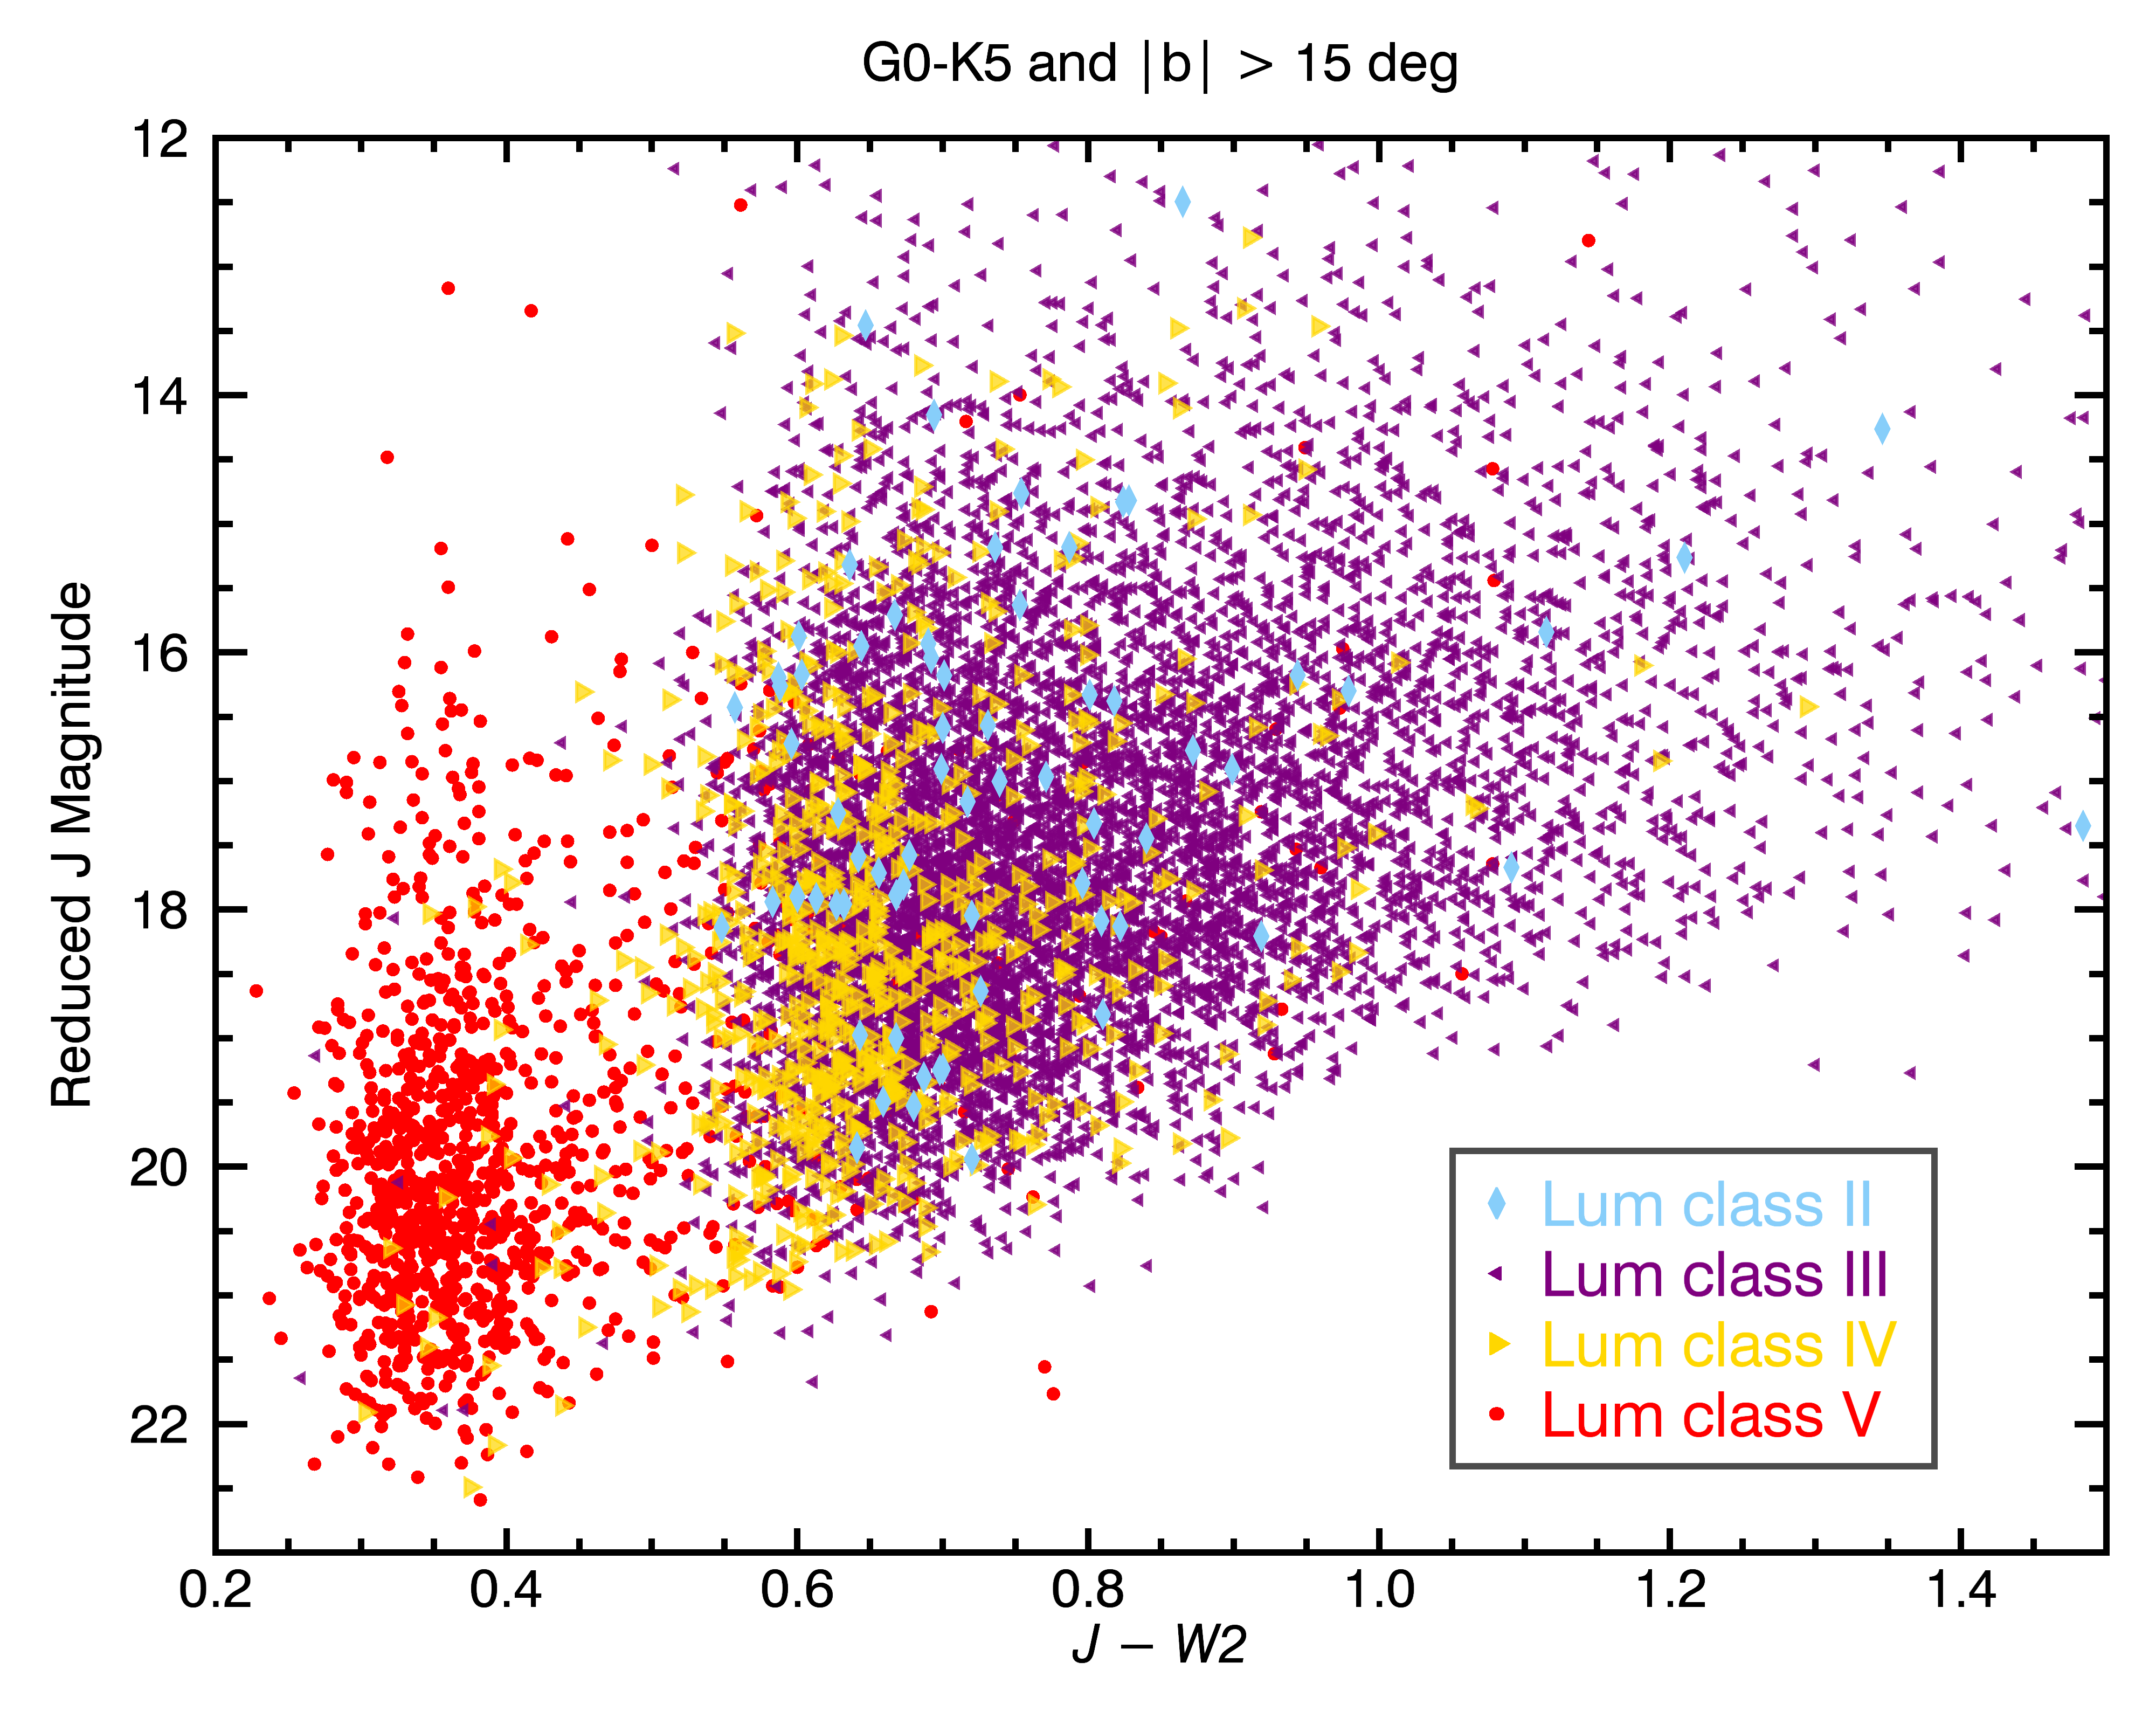
\includegraphics[width=1.0\textwidth,clip=true]{Figures/absolute_j/plot-J-W2-G0-K5-b15-0.png}
 \end{center}
 \caption{Reduced $J$-band proper motion plot using \textit{GAIA} DR1 proper motions as a function of $J-W2$ color for Michigan Spectral Atlas stars with spectra types between G0 and K5 and galactic latitudes $|b|>15\deg$.  The different colors correspond to the different luminosity classes, and show a relatively clear separation between dwarfs and (sub-)giants.}
\end{figure*}

\begin{figure*}[t]
  \begin{center}
      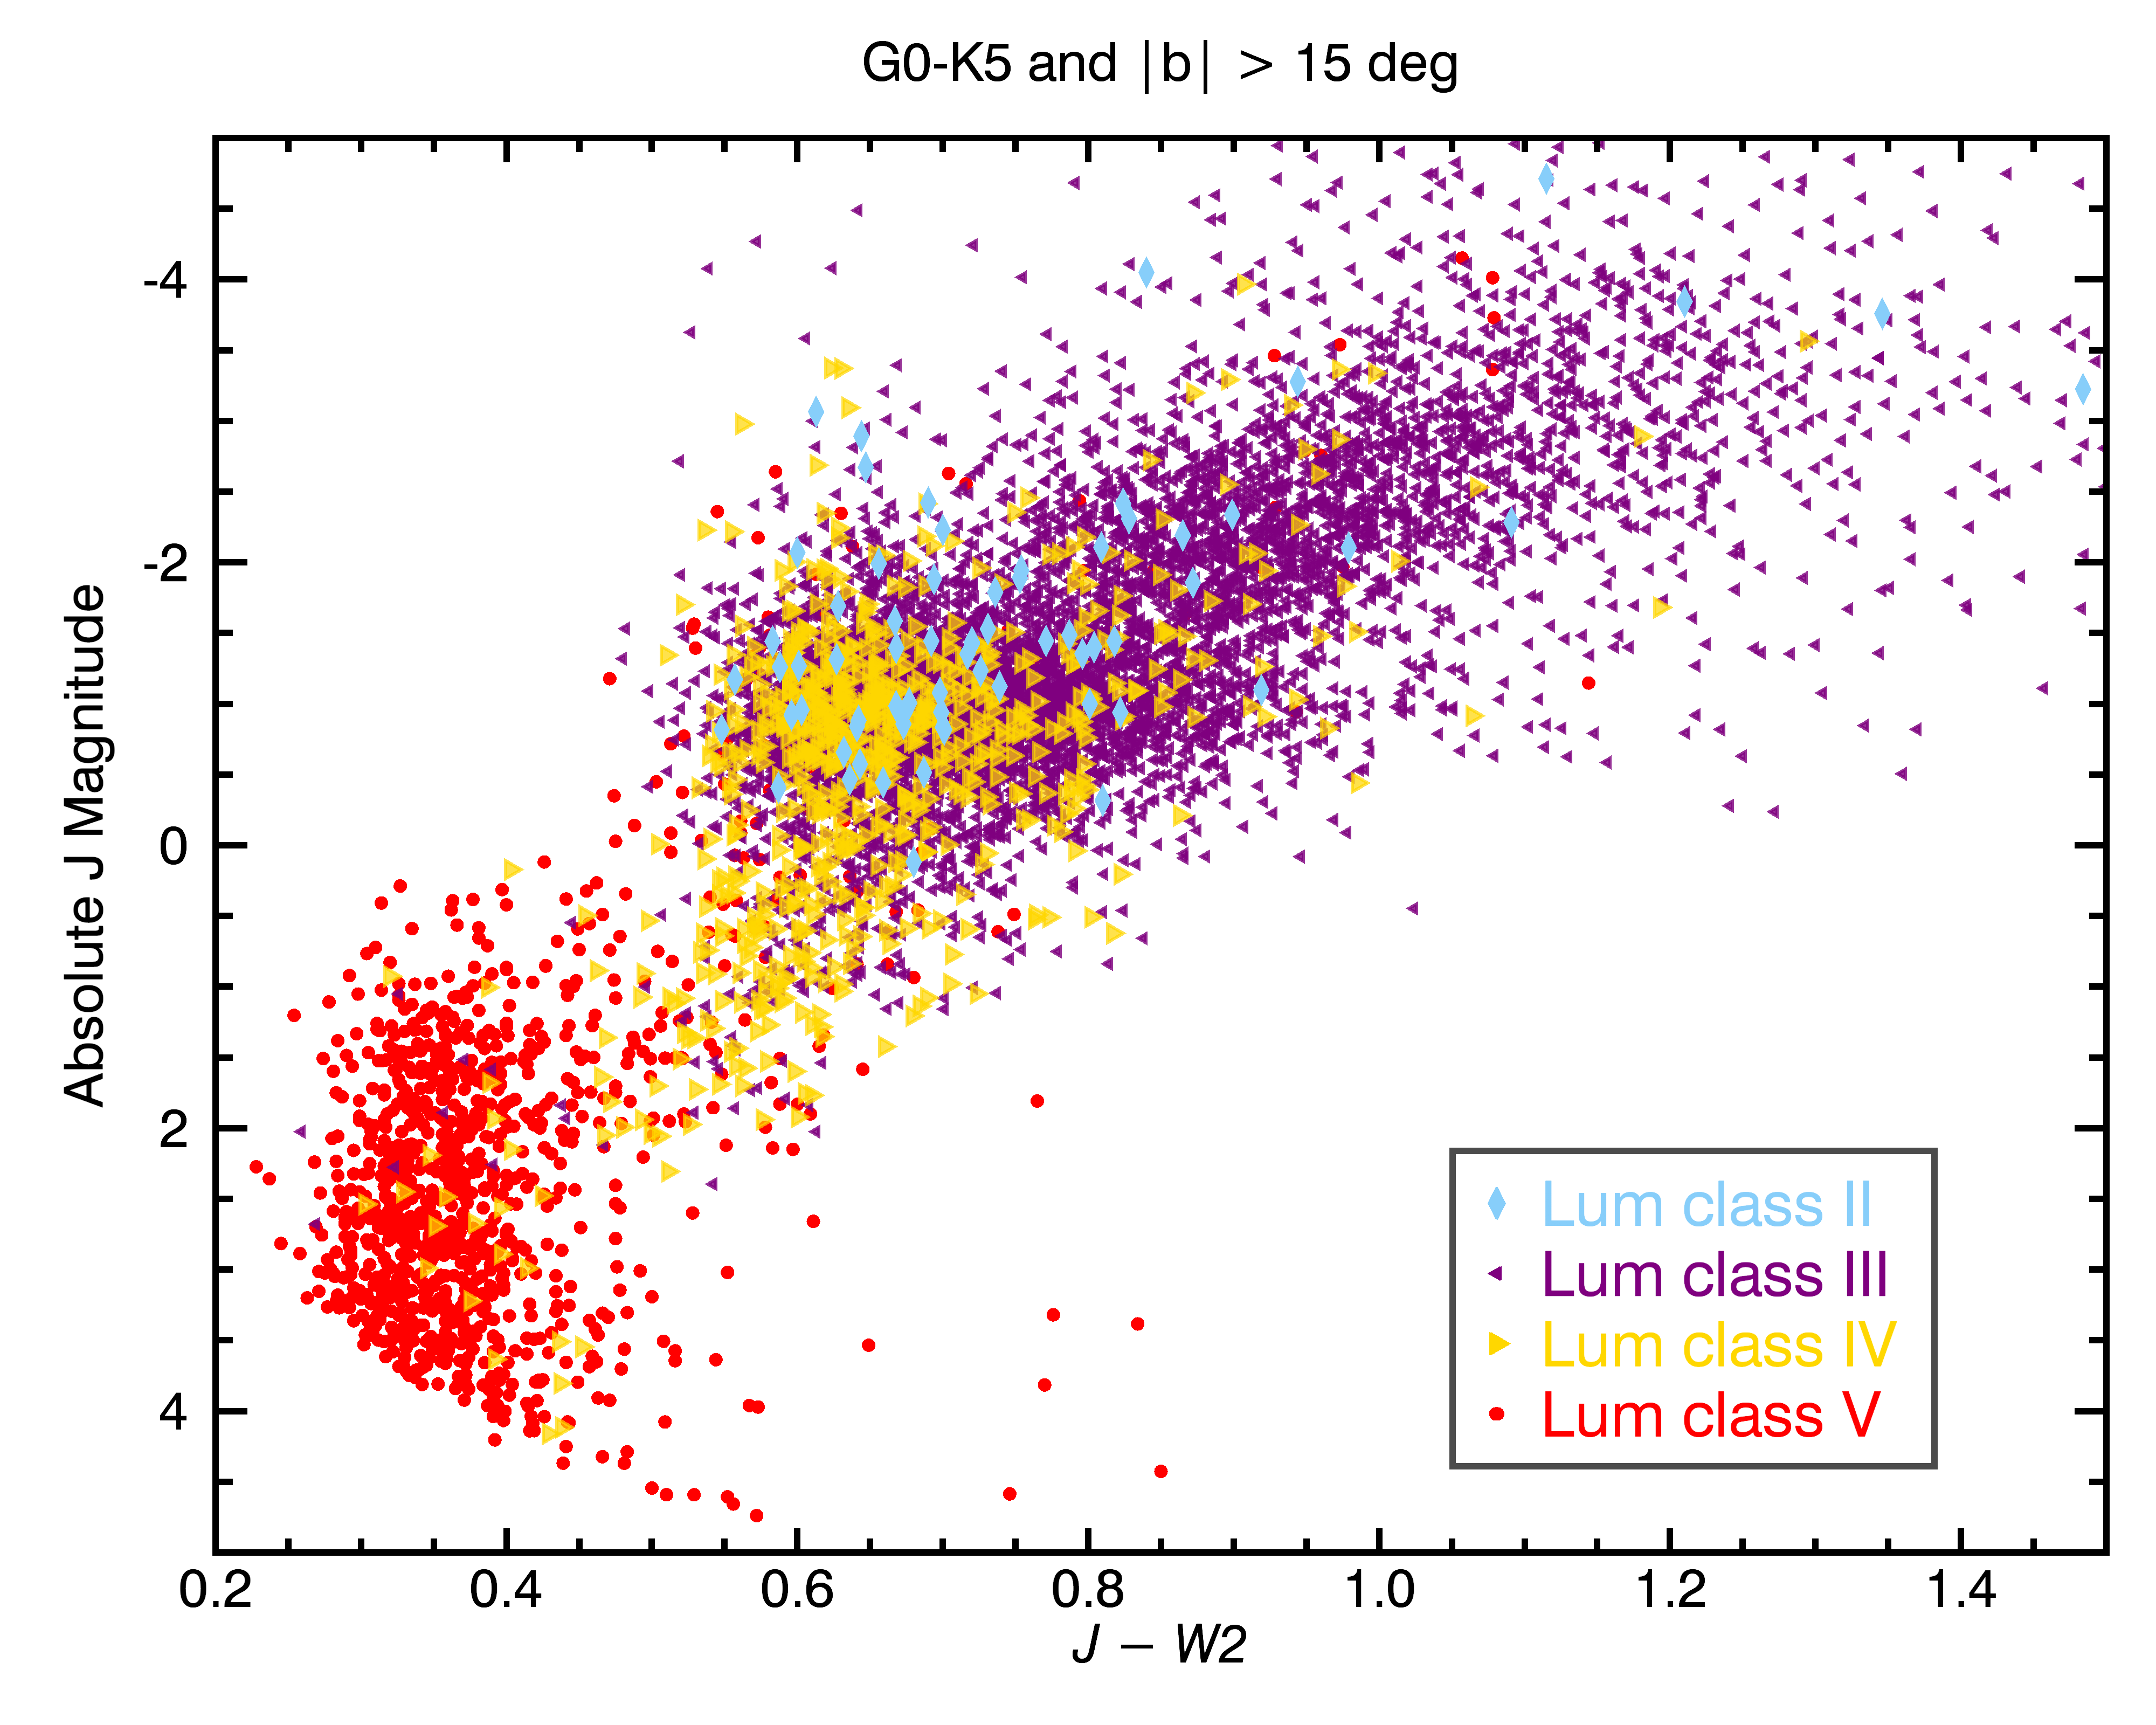
\includegraphics[width=1.0\textwidth,clip=true]{Figures/absolute_j/plot-J-W2-G0-K5-b15-1.png}
 \end{center}
 \caption{The same as the previous figure, but for absolute $J$ band magnitudes using \textit{GAIA} DR1 parallaxes, validating the Michigan Spectral Atlas luminosity classes and the reduced proper motion approach.}
\end{figure*}

We are considering also further finessing the color-luminosity class probability by relating color with position in the sky using a a synthetic galactic model of the Milky Way called TRILEGAL, but leave this for future work. Incorporating giant/dwarf population statistics, such as luminosity class number density as a function sky area, should help to further improve color as a tool to predict luminosity class, and for application to future surveys.

We pick an ecliptic pole field as an application of calculating probabilistic luminosity class membership in a Bayesian framework.

In particular, our priors are the mean and robust standard deviation of colors of each luminosity class. We use the TRILEGAL source counts to normalize these distributions with respect to one another, and integrate over a sample photometric measurement and its uncertainty.

